\chapter{Optimasi Konveks dan Dualitas}

Sebuah pencampur warna bekerja dengan dua pigmen. Tiap pigmen punya takaran yang paling
disukai mesin: dua bagian untuk pigmen pertama, dua bagian untuk pigmen kedua. Tetapi
resep menuntut jumlah keduanya tepat dua bagian, dan kelarutan pigmen pertama tidak
mengizinkan lebih dari setengah bagian. Kita ingin campuran yang sedekat mungkin dengan
kesukaan mesin, dengan dua tuntutan yang tidak bisa dilanggar. Tanpa tuntutan, jawabannya
dua dan dua; dengan tuntutan jumlah saja, satu dan satu. Tuntutan kelarutan menggeser
jawaban lagi, dan tidak jelas lagi ke arah mana.

Bentuk soal itu muncul di tempat yang tidak berbau pigmen. Dua bobot model punya nilai
terbaik dari pencocokan sebelumnya, sebuah syarat kalibrasi menuntut jumlah keduanya
tetap, dan satu pembatas perangkat membatasi salah satunya. Berapa bobot terbaik yang
masih memenuhi keduanya, dan berapa harga tiap tuntutan dalam satuan fungsi sasaran?
Pertanyaan kedua itu yang dipakai insinyur untuk memutuskan tuntutan mana yang layak
dilonggarkan.

Bab 10 memberi kuadrat terkecil, tetapi hanya tanpa kendala. Bab 12 memberi gradien, tetapi
gradien hanya berbicara tentang tetangga: titik dengan gradien nol bisa minimum, maksimum,
atau pelana. Bab 9 memberi nilai eigen, yang dipakai di sini, tetapi nilai eigen tidak
menjawab pertanyaan terpenting: kalau algoritme berhenti di suatu titik, apakah itu
jawaban terbaik di seluruh daerah layak? Untuk fungsi konveks ya. Untuk soal umum tidak,
dan bagian keempat menunjukkan bagaimana dualitas memberi batas bawah yang sah tanpa
memeriksa seluruh daerah layak.

\begin{untukanak}
Pernahkah kamu menaruh kelereng di dalam mangkuk? Kelereng itu selalu berhenti di dasar, di
tempat yang sama, ke mana pun ia dilepas, karena dasarnya cekung ke atas seperti huruf U.
Sekarang bayangkan kelereng yang sama dilepas di lereng bukit berbatu. Ia berhenti di
lekukan pertama yang cukup dalam, dan lekukan itu belum tentu yang paling rendah. Dari
tempat berhenti, kamu tidak bisa tahu apakah ada lembah lain yang lebih dalam tanpa
berjalan jauh dan memeriksa.

Di bab ini kita akan tahu mengapa mangkuk begitu bersahabat dan bukit begitu menipu, dan
mengapa kita bisa membedakan keduanya sebelum menghitung apa pun. Ada gagasan kedua yang
lebih halus: kadang kita tidak perlu tahu letak dasar lembah, cukup tahu batas terendah
yang mungkin dicapai. Kalau batas itu sama dengan tempat kita berdiri, kita yakin tidak
ada yang lebih baik, tanpa memeriksa satu titik pun. Batas semacam itu dijual oleh daftar
harga untuk setiap tuntutan, dan daftar harga itulah yang membuat banyak soal optimasi
bisa dipercaya tanpa diselesaikan sampai habis.
\end{untukanak}

\section{Himpunan konveks dan kombinasi konveks}
\tingkat{dasar}

Kata ``konveks'' dalam bahasa sehari-hari berarti cembung ke luar, seperti punggung
kura-kura. Dalam optimasi artinya hampir kebalikannya: himpunan disebut konveks bila ia
tidak punya lekuk ke dalam, sehingga ruas garis antara dua anggotanya tetap di dalam.
Mangkuk tadi konveks; daerah di antara dua tanduk bulan tidak.

Aturan mainnya satu: campur dua titik dengan bobot tak negatif yang jumlahnya satu, dan
hasil campuran itu harus tetap anggota himpunan. Bobot satu berarti memilih titik pertama, bobot
nol titik kedua, bobot setengah tepat di tengah.

\kamus{kombinasi konveks}{convex combination}{Resep mencampur beberapa titik dengan
takaran yang jumlahnya tepat satu, seperti mencampur cat: hasilnya selalu di antara
bahan-bahannya.}

\begin{definisi}[Himpunan konveks dan kombinasi konveks]
Himpunan $C\subseteq\mathbb{R}^{n}$ disebut \emph{konveks} bila untuk setiap
$\mathbf{x},\mathbf{y}\in C$ dan setiap $t\in[0,1]$ berlaku
$t\mathbf{x}+(1-t)\mathbf{y}\in C$. Titik itu disebut \emph{kombinasi konveks} dari
$\mathbf{x}$ dan $\mathbf{y}$. Secara umum, $\sum_{i=1}^{k}\theta_{i}\mathbf{x}_{i}$
disebut kombinasi konveks bila $\theta_{i}\ge0$ dan $\sum_{i}\theta_{i}=1$.
\emph{Selubung konveks} $\operatorname{conv}S$ adalah himpunan semua kombinasi konveks
berhingga titik di $S$.\index{himpunan konveks}\index{kombinasi konveks}
\end{definisi}

Definisi dengan dua titik cukup untuk semua titik: bila $C$ memuat setiap campuran dua
anggota, ia memuat setiap campuran berhingga anggotanya, dengan induksi pada banyak
titik.

Empat contoh penting. \emph{Hiperbidang}
$\{\mathbf{x}:\mathbf{a}^{\top}\mathbf{x}=b\}$ konveks, sebab
$\mathbf{a}^{\top}(t\mathbf{x}+(1-t)\mathbf{y})=tb+(1-t)b=b$. \emph{Setengah ruang}
$\{\mathbf{x}:\mathbf{a}^{\top}\mathbf{x}\le b\}$ konveks dengan alasan yang sama memakai
ketaksamaan. \emph{Bola} $\{\mathbf{x}:\|\mathbf{x}-\mathbf{c}\|\le r\}$ konveks karena
norma memenuhi ketaksamaan segitiga (Bab 10):
\[
  \|t\mathbf{x}+(1-t)\mathbf{y}-\mathbf{c}\|
  \le t\|\mathbf{x}-\mathbf{c}\|+(1-t)\|\mathbf{y}-\mathbf{c}\|\le tr+(1-t)r=r .
\]
\emph{Polihedron}, yaitu irisan berhingga hiperbidang dan setengah ruang, konveks karena
alasan berikut.

\begin{proposisi}[Irisan mempertahankan konveksitas]
Bila $C_{1},\dots,C_{k}$ konveks, maka $\bigcap_{i=1}^{k}C_{i}$ konveks.
\end{proposisi}

\begin{proof}
Ambil $\mathbf{x},\mathbf{y}$ di irisan dan $t\in[0,1]$. Untuk setiap $i$, kedua titik
itu anggota $C_{i}$, jadi $t\mathbf{x}+(1-t)\mathbf{y}\in C_{i}$ karena $C_{i}$ konveks.
Karena itu titik campuran berada di setiap $C_{i}$, yaitu di irisan.
\end{proof}

Irisan murah hati; gabungan tidak. Ambil $C_{1}=\{(x_{1},0):x_{1}\in[0,1]\}$ dan
$C_{2}=\{(x_{1},1):x_{1}\in[0,1]\}$, keduanya konveks. Titik $(0,0)$ dan $(0,1)$ ada di
gabungan, tetapi campuran setengahnya $(0,\tfrac12)$ tidak. Hal yang sama terjadi pada
$\{(x_{1},x_{2}):x_{1}x_{2}\ge1\}$: titik $(-1,-1)$ dan $(1,1)$ keduanya anggota,
sedangkan titik asal bukan, sebab $0<1$. Himpunan itu dua daerah terpisah.

Selubung konveks adalah tambalan termurah untuk lubang semacam itu: himpunan konveks
terkecil yang memuat $S$. Ia selalu ada, karena irisan semua himpunan konveks yang memuat
$S$ konveks menurut proposisi tadi dan tidak kosong, sebab $\mathbb{R}^{n}$ sendiri
konveks.

\section{Fungsi konveks dan dua ujinya}
\tingkat{menengah}

Himpunan konveks berbicara tentang daerah; fungsi konveks berbicara tentang bentuk
permukaan di atas daerah itu. Yang dituntut: nilai di titik campuran tidak lebih besar
daripada campuran nilai. Pada Gambar~\ref{fig:fungsi-konveks} kiri, tali dari $(-1,1)$ ke
$(1,1)$ di atas grafik $f(t)=t^{2}$; pada panel kanan talinya terpotong.

\kamus{fungsi konveks}{convex function}{Permukaan yang tidak pernah melengkung ke atas
seperti atap; tali antar dua titiknya selalu di atas permukaan.}

\begin{definisi}[Fungsi konveks]
Misalkan $C\subseteq\mathbb{R}^{n}$ konveks. Fungsi $f\colon C\to\mathbb{R}$ disebut
\emph{konveks} bila
\[
  f\bigl(t\mathbf{x}+(1-t)\mathbf{y}\bigr)
  \le t\,f(\mathbf{x})+(1-t)\,f(\mathbf{y})
\]
untuk semua $\mathbf{x},\mathbf{y}\in C$ dan $t\in[0,1]$. Ia \emph{konveks ketat} bila
ketaksamaan itu ketat untuk $\mathbf{x}\ne\mathbf{y}$ dan $t\in(0,1)$, dan \emph{cekung}
bila $-f$ konveks.\index{fungsi konveks}
\end{definisi}

\begin{figure}[!ht]
\centering
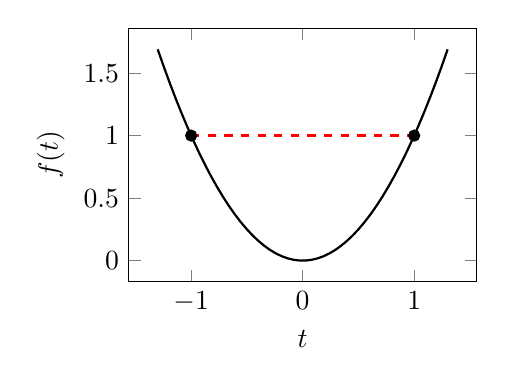
\begin{tikzpicture}
\begin{axis}[width=6cm,height=4.8cm,xlabel={$t$},ylabel={$f(t)$}]
\addplot[domain=-1.3:1.3,samples=50,thick] {x^2};
\addplot[dashed,thick,red] coordinates {(-1,1) (1,1)};
\addplot[only marks,mark=*] coordinates {(-1,1) (1,1)};
\end{axis}
\end{tikzpicture}\quad
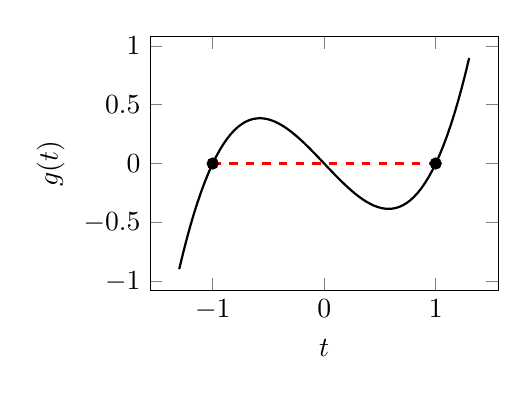
\begin{tikzpicture}
\begin{axis}[width=6cm,height=4.8cm,xlabel={$t$},ylabel={$g(t)$}]
\addplot[domain=-1.3:1.3,samples=80,thick] {x^3-x};
\addplot[dashed,thick,red] coordinates {(-1,0) (1,0)};
\addplot[only marks,mark=*] coordinates {(-1,0) (1,0)};
\end{axis}
\end{tikzpicture}
\caption{Tali antara dua titik grafik. Kiri: $f(t)=t^{2}$, tali dari $(-1,1)$ ke $(1,1)$
bernilai $1$ di $t=0$ sedangkan grafiknya $0$, jadi tali di atas grafik. Kanan:
$g(t)=t^{3}-t$, tali dari $(-1,0)$ ke $(1,0)$ memotong grafik di $t=-1$, $0$, $1$; di
$t=-0{,}5$ grafik bernilai $0{,}375$ sedangkan talinya $0$.}
\label{fig:fungsi-konveks}
\end{figure}

Definisi itu setara dengan pernyataan geometris tentang \emph{epigraf}, yaitu himpunan
titik di atas grafik: $f$ konveks tepat ketika
$\operatorname{epi}f=\{(\mathbf{x},t):f(\mathbf{x})\le t\}$ konveks. Kesetaraannya murni
aljabar, dan memindahkan pertanyaan tentang fungsi menjadi pertanyaan tentang himpunan.

Untuk fungsi yang dapat diturunkan ada dua uji yang jauh lebih cepat, dan keduanya
perlu-dan-cukup, bukan hanya cukup.

\begin{teorema}[Uji orde pertama]
Misalkan $f$ terdiferensialkan pada himpunan konveks terbuka $C$. Fungsi $f$ konveks jika
dan hanya jika
\[
  f(\mathbf{y})\ge f(\mathbf{x})+\nabla f(\mathbf{x})^{\top}(\mathbf{y}-\mathbf{x})
\]
untuk semua $\mathbf{x},\mathbf{y}\in C$.
\end{teorema}

\begin{proof}
Andaikan $f$ konveks, ambil $\mathbf{x}\ne\mathbf{y}$ dan $t\in(0,1)$. Dari definisi,
\[
  \frac{f\bigl(\mathbf{x}+t(\mathbf{y}-\mathbf{x})\bigr)-f(\mathbf{x})}{t}
  \le f(\mathbf{y})-f(\mathbf{x}).
\]
Saat $t\downarrow0$ ruas kiri menuju turunan berarah
$\nabla f(\mathbf{x})^{\top}(\mathbf{y}-\mathbf{x})$, sehingga ketaksamaan yang diminta
tercapai di limit. Untuk arah sebaliknya, andaikan ketaksamaan itu berlaku dan ambil
$\mathbf{z}=t\mathbf{x}+(1-t)\mathbf{y}$ dengan $t\in[0,1]$. Terapkan ketaksamaan di
$\mathbf{z}$ terhadap $\mathbf{x}$ dan terhadap $\mathbf{y}$:
\[
  f(\mathbf{x})\ge f(\mathbf{z})+\nabla f(\mathbf{z})^{\top}(\mathbf{x}-\mathbf{z}),
  \qquad
  f(\mathbf{y})\ge f(\mathbf{z})+\nabla f(\mathbf{z})^{\top}(\mathbf{y}-\mathbf{z}).
\]
Kalikan yang pertama dengan $t$, yang kedua dengan $1-t$, lalu jumlahkan. Suku gradien
lenyap karena $t(\mathbf{x}-\mathbf{z})+(1-t)(\mathbf{y}-\mathbf{z})=\mathbf{0}$, dan
tersisa $t\,f(\mathbf{x})+(1-t)f(\mathbf{y})\ge f(\mathbf{z})$.
\end{proof}

Bacaan praktisnya: grafiknya di atas setiap bidang singgung. Satu bidang singgung sudah
memberi batas bawah global, dan itulah sebabnya gradien di titik mana pun menjadi alat
yang jujur, bukan ramalan lokal.

\begin{teorema}[Uji orde kedua]
Misalkan $f$ terdiferensialkan dua kali pada himpunan konveks terbuka $C$. Fungsi $f$
konveks jika dan hanya jika Hessian $\nabla^{2}f(\mathbf{x})$ semidefinit positif untuk
setiap $\mathbf{x}\in C$, yaitu
$\mathbf{v}^{\top}\nabla^{2}f(\mathbf{x})\mathbf{v}\ge0$ untuk semua $\mathbf{v}$.
\index{Hessian}
\end{teorema}

\begin{proof}
Bila $f$ konveks, untuk setiap $\mathbf{x}$ dan $\mathbf{v}$ fungsi satu variabel
$g(s)=f(\mathbf{x}+s\mathbf{v})$ konveks pada selang di sekitar nol, sebab komposisi
dengan peta afin mempertahankan konveksitas. Uji orde pertama pada $g$ menunjukkan $g'$
naik, sehingga $g''(0)\ge0$; dan $g''(0)=\mathbf{v}^{\top}\nabla^{2}f(\mathbf{x})
\mathbf{v}$.

Sebaliknya, bila Hessian semidefinit positif di seluruh $C$, teorema Taylor dengan sisa
integral (Bab 12) memberi
\[
  f(\mathbf{y})=f(\mathbf{x})+\nabla f(\mathbf{x})^{\top}(\mathbf{y}-\mathbf{x})
  +\int_{0}^{1}(1-s)\,(\mathbf{y}-\mathbf{x})^{\top}
   \nabla^{2}f\bigl(\mathbf{x}+s(\mathbf{y}-\mathbf{x})\bigr)(\mathbf{y}-\mathbf{x})\,ds .
\]
Integran tidak negatif karena Hessian semidefinit positif dan $(1-s)\ge0$, jadi suku
integralnya tidak negatif. Ketaksamaan orde pertama terpenuhi, dan $f$ konveks.
\end{proof}

Dua peringatan tentang uji orde kedua. Pertama, Hessian \emph{definit} positif cukup
untuk konveks ketat, tetapi bukan syarat perlu: $f(x)=x^{4}$ konveks ketat padahal
$f''(0)=0$. Kedua, Hessian semidefinit positif hanya memberi konveksitas, bukan ketatnya;
$f(x_{1},x_{2})=x_{1}^{2}$ punya Hessian $\operatorname{diag}(2,0)$ dan minimumnya
seluruh garis $x_{1}=0$.

\begin{bacakeras}
Dua suara, dibaca bergantian dengan teman. Suara pertama bertanya, suara kedua menjawab.

``Aku menjatuhkan kelereng di mangkuk. Ke mana ia pergi?'' ``Ke dasar. Selalu ke dasar
yang sama.'' ``Kalau aku melepasnya dari sisi yang lain?'' ``Ke dasar itu juga.'' ``Jadi
hanya ada satu tempat terendah?'' ``Hanya satu, dan setiap jalan menurun menemukannya.''

``Sekarang aku melepasnya di lereng batu. Ke mana ia pergi?'' ``Ke lekukan pertama yang
cukup dalam.'' ``Apakah itu yang terdalam?'' ``Belum tentu. Lekukan itu menahannya, bukan
meyakinkannya.''

Ulangi bergantian, makin cepat, dengan ketukan meja: mangkuk tidak punya jebakan, bukit
punya jebakan.

Baris yang harus diulang pembaca, sekali, dengan suara jelas: kalau setiap jalan menurun
berakhir di titik yang sama, di situ tidak ada jebakan, dan itulah arti konveks.
\end{bacakeras}

Beberapa operasi mempertahankan konveksitas. Jumlah dua fungsi konveks tetap konveks,
karena ketaksamaannya dijumlahkan; kelipatan positif juga. Komposisi
$f(\mathbf{A}\mathbf{x}+\mathbf{b})$ konveks bila $f$ konveks, sebab peta afin memetakan
campuran ke campuran. Maksimum titik demi titik juga konveks: bila $f=\max_{i}f_{i}$,
ketaksamaan bagi setiap $f_{i}$ berlaku bagi maksimumnya. Itu menjelaskan mengapa
$\max\{|x_{1}|,|x_{2}|\}$ berpatahan tetapi tetap konveks.

\begin{resep}
Empat langkah memeriksa kecembungan, dari yang paling murah.
\begin{enumerate}
  \item Periksa daerahnya lebih dulu: ambil dua titik di $C$ dan pastikan ruas di
        antaranya tetap di $C$. Bila gagal, berhenti, karena uji berikutnya mengandaikan
        $C$ konveks.
  \item Uji lewat definisi dengan pasangan umum $\mathbf{x},\mathbf{y}$: tulis
        $f(t\mathbf{x}+(1-t)\mathbf{y})$ dan bandingkan dengan
        $t\,f(\mathbf{x})+(1-t)f(\mathbf{y})$ untuk $t\in[0,1]$. Satu pasangan yang
        membalik ketaksamaan sudah cukup untuk menolak.
  \item Hitung Hessian $\nabla^{2}f(\mathbf{x})$ sebagai fungsi $\mathbf{x}$, bukan satu
        matriks angka di satu titik.
  \item Putuskan tandanya: nilai eigen tak negatif, atau semua minor utama
        $1\times1$ sampai $n\times n$ tak negatif. Satu nilai eigen negatif sudah
        menutup perkara.
\end{enumerate}
Peringatan urutan: langkah 4 tidak boleh dikerjakan sebelum langkah 1. Hessian yang
definit positif di satu titik hanya berbicara tentang titik itu, sedangkan definisi
berbicara tentang seluruh $C$.
\end{resep}

\section{Bentuk baku dan mengapa optimum lokal menjadi global}
\tingkat{menengah}

Sampai sini kita punya dua gagasan terpisah: daerah yang tidak berlubang dan permukaan
yang tidak melengkung ke atas. Optimasi menyatukan keduanya lewat satu bentuk tulisan.
Setiap masalah optimasi dapat ditulis dengan cara yang sama: satu fungsi yang hendak
dikecilkan, sekumpulan syarat ketaksamaan, dan sekumpulan syarat kesamaan.

\kamus{bentuk baku}{standard form}{Cara menulis semua soal optimasi dengan satu pola:
satu sasaran, syarat ``tidak lebih dari nol'', dan syarat ``sama dengan''.}

\begin{definisi}[Masalah optimasi bentuk baku]
\emph{Masalah optimasi bentuk baku} adalah
\[
  \begin{array}{ll}
  \text{minimumkan} & f_{0}(\mathbf{x})\\
  \text{dengan} & f_{i}(\mathbf{x})\le0,\qquad i=1,\dots,m,\\
                & h_{j}(\mathbf{x})=0,\qquad j=1,\dots,p,
  \end{array}
\]
dengan variabel $\mathbf{x}\in\mathbb{R}^{n}$, fungsi sasaran $f_{0}$, fungsi kendala
ketaksamaan $f_{i}$, dan fungsi kendala kesamaan $h_{j}$. Daerah asalnya
$D=\bigcap_{i}\operatorname{dom}f_{i}\cap\bigcap_{j}\operatorname{dom}h_{j}$, daerah
layaknya $X=\{\mathbf{x}\in D:f_{i}(\mathbf{x})\le0,\ h_{j}(\mathbf{x})=0\}$, dan
\emph{nilai optimum} $p^{*}=\inf_{\mathbf{x}\in X}f_{0}(\mathbf{x})$, boleh
$-\infty$ bila masalahnya tak terbatas ke bawah. Masalahnya disebut \emph{masalah
konveks} bila $f_{0},\dots,f_{m}$ konveks dan $h_{1},\dots,h_{p}$ afin.
\index{bentuk baku}
\end{definisi}

Bahwa setiap kendala dapat dibawa ke pola ini mudah diperiksa. Syarat
$f(\mathbf{x})\ge b$ menjadi $b-f(\mathbf{x})\le0$; kesamaan linear tetap kesamaan;
memaksimumkan $f$ sama dengan meminimumkan $-f$. Yang tidak gratis hanyalah konveksitas:
membalik tanda ketaksamaan membalik konveksitas fungsinya, jadi arah ketaksamaan tidak
boleh diubah tanpa memeriksa ulang.

\begin{akibat}[Daerah layak konveks]
Pada masalah konveks, daerah layak $X$ konveks.
\end{akibat}

\begin{proof}
Himpunan bawah $S_{i}=\{\mathbf{x}:f_{i}(\mathbf{x})\le0\}$ konveks untuk setiap $i$:
bila $f_{i}(\mathbf{x})\le0$ dan $f_{i}(\mathbf{y})\le0$, konveksitas memberi
$f_{i}(t\mathbf{x}+(1-t)\mathbf{y})\le t\,f_{i}(\mathbf{x})+(1-t)f_{i}(\mathbf{y})\le0$.
Himpunan $\{\mathbf{x}:h_{j}(\mathbf{x})=0\}$ adalah hiperbidang karena $h_{j}$ afin,
jadi konveks. Daerah layak adalah irisan semuanya, dan irisan himpunan konveks juga konveks
menurut proposisi di bagian pertama.
\end{proof}

Akibat itu yang membuat seluruh bab ini masuk akal: dua titik layak selalu bisa
dihubungkan tanpa keluar dari daerah layak. Bentuk paling sederhana polihedron adalah
daerah layak program linear dua variabel pada Gambar~\ref{fig:lp-verteks}: segi empat,
dan sasaran linearnya optimal di verteks.

\begin{figure}[!ht]
\centering
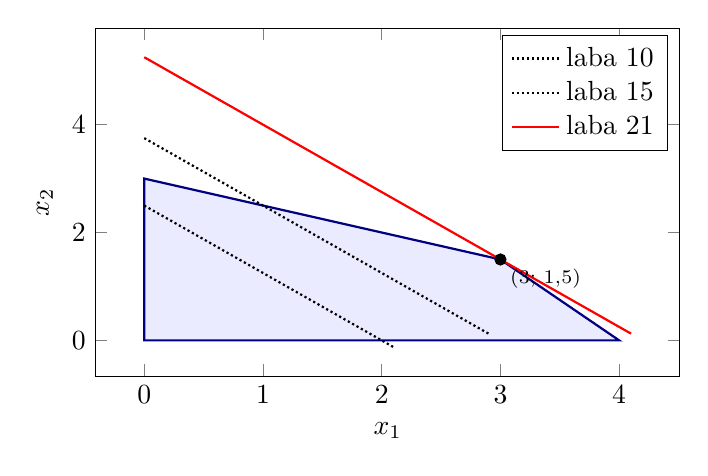
\begin{tikzpicture}
\begin{axis}[width=9cm,height=6cm,xlabel={$x_{1}$},ylabel={$x_{2}$}]
\addplot[forget plot,fill=blue!8,draw=blue!50!black,thick]
  coordinates {(0,0) (4,0) (3,1.5) (0,3)} \closedcycle;
\addplot[domain=0:2.1,densely dotted,thick] {2.5-1.25*x};
\addlegendentry{laba $10$}
\addplot[domain=0:2.9,densely dotted,thick] {3.75-1.25*x};
\addlegendentry{laba $15$}
\addplot[domain=0:4.1,thick,red] {5.25-1.25*x};
\addlegendentry{laba $21$}
\addplot[forget plot,only marks,mark=*] coordinates {(3,1.5)};
\node[font=\scriptsize,below right] at (axis cs:3,1.5) {$(3;\,1{,}5)$};
\end{axis}
\end{tikzpicture}
\caption{Daerah layak program linear bengkel Bab 24: $6x_{1}+4x_{2}\le24$ (kayu lapis),
$x_{1}+2x_{2}\le6$ (jam), $x_{1},x_{2}\ge0$, sasaran $5x_{1}+4x_{2}$. Verteks
$(0;0)$, $(4;0)$, $(3;1{,}5)$, $(0;3)$ bernilai $0$, $20$, $21$, $12$. Garis level $21$
hanya menyentuh verteks $(3;1{,}5)$; garis $20$ masih memotong daerah layak.}
\label{fig:lp-verteks}
\end{figure}


Sekarang pernyataan yang dijanjikan pembuka bab, dan buktinya pendek justru karena
daerah layak konveks.

\begin{teorema}[Minimum lokal adalah minimum global]
Misalkan $f_{0}$ konveks pada himpunan konveks $X$, dan $\mathbf{x}^{*}\in X$ memenuhi
$f_{0}(\mathbf{x}^{*})\le f_{0}(\mathbf{x})$ untuk semua $\mathbf{x}\in X$ yang cukup
dekat dengan $\mathbf{x}^{*}$. Maka $f_{0}(\mathbf{x}^{*})\le f_{0}(\mathbf{x})$ untuk
semua $\mathbf{x}\in X$. Himpunan semua titik minimum juga konveks.
\index{optimum global}
\end{teorema}

\begin{proof}
Andaikan ada $\mathbf{y}\in X$ dengan $f_{0}(\mathbf{y})<f_{0}(\mathbf{x}^{*})$. Untuk
$t\in(0,1]$ titik $\mathbf{z}_{t}=(1-t)\mathbf{x}^{*}+t\mathbf{y}$ berada di $X$ dan
memusat ke $\mathbf{x}^{*}$ saat $t\to0$, jadi untuk $t$ cukup kecil ia masuk ke
tetangga tempat $\mathbf{x}^{*}$ minimum lokal. Tetapi konveksitas memberi
\[
  f_{0}(\mathbf{z}_{t})\le(1-t)f_{0}(\mathbf{x}^{*})+t\,f_{0}(\mathbf{y})
  <f_{0}(\mathbf{x}^{*}),
\]
bertentangan dengan keminimuman lokal. Untuk bagian kedua, bila
$\mathbf{x}^{*},\mathbf{y}^{*}$ keduanya minimum bernilai $p^{*}$, maka
$f_{0}(\mathbf{z}_{t})\le p^{*}$, sedangkan $p^{*}$ adalah nilai terkecil yang mungkin,
jadi $f_{0}(\mathbf{z}_{t})=p^{*}$ dan $\mathbf{z}_{t}$ juga minimum.
\end{proof}

\begin{akibat}[Syarat stasioner tanpa kendala]
Bila $f$ konveks dan terdiferensialkan pada himpunan terbuka, maka
$\nabla f(\mathbf{x}^{*})=\mathbf{0}$ jika dan hanya jika $\mathbf{x}^{*}$ minimum
global.
\end{akibat}

\begin{proof}
Bila $\nabla f(\mathbf{x}^{*})=\mathbf{0}$, uji orde pertama memberi
$f(\mathbf{y})\ge f(\mathbf{x}^{*})$ untuk setiap $\mathbf{y}$. Sebaliknya, bila
$\mathbf{x}^{*}$ minimum, maka untuk setiap arah $\mathbf{v}$ dan $t>0$ kecil berlaku
$f(\mathbf{x}^{*}+t\mathbf{v})\ge f(\mathbf{x}^{*})$, sehingga turunan berarahnya
$\nabla f(\mathbf{x}^{*})^{\top}\mathbf{v}\ge0$. Karena $\mathbf{v}$ juga boleh diganti
$-\mathbf{v}$, haruslah $\nabla f(\mathbf{x}^{*})=\mathbf{0}$.
\end{proof}

\begin{tangan}
Bahan: tali dua meter, satu cincin kecil, penutup mata, dan seorang teman.

Ikat tali pada dua tiang setinggi sama, lalu regangkan sampai lurus. Minta teman menutup
mata, menggantungkan cincin di tengah tali, dan menggesernya perlahan ke kiri dan ke
kanan dengan satu jari. Cincin meluncur ke titik terendah, ke mana pun ia dilepas. Minta
teman menandai titik berhentinya tanpa membuka mata; ulangi lima kali dari posisi awal
berbeda. Semua tanda harus jatuh pada satu titik.

Sekarang ikat satu simpul kecil di tali, agak ke kiri, sehingga talinya membentuk dua
lekuk. Ulangi percobaan. Cincin berhenti di lekuk kiri bila dilepas di dekat situ, dan
di tengah bila dilepas di kanan simpul: dua tempat berhenti, dua lembah.

Yang harus terlihat: tali tanpa simpul hanya punya satu titik terendah, tali bersimpul
punya dua, dan jari yang berhenti di lekuk kiri tidak tahu apa yang terjadi di kanan,
persis seperti algoritme yang berhenti di titik stasioner pertama.
\end{tangan}

Tanpa konveksitas, akibat itu salah. Ambil $f(x_{1},x_{2})=x_{1}x_{2}$ pada bujur
sangkar $[-1,1]^{2}$. Gradiennya $(x_{2},x_{1})$ lenyap di titik asal, padahal
$f(\mathbf{0})=0$ sedangkan $f(1,-1)=-1$. Hessiannya
$\begin{pmatrix}0&1\\1&0\end{pmatrix}$ dengan nilai eigen $1$ dan $-1$, jadi uji orde
kedua menolak konveksitas: titik asal pelana, bukan lembah. Bab 24 memberi contoh yang
lebih menipu: pembulatan jawaban bersambung memberi laba 19, padahal jawaban bulat
terbaik memberi 20.

\section{Lagrangian dan batas bawah dari dual}
\tingkat{lanjut}

Kendala selalu berbentuk ``sesuatu tidak boleh positif'', jadi kita bisa memberi harga
pada pelanggaran: setiap kali $f_{i}(\mathbf{x})$ positif, kita membayar denda
$\lambda_{i}$ per satuan, dan setiap penyimpangan $h_{j}(\mathbf{x})$ dari nol dibayar
atau diterima sebesar $\nu_{j}$ per satuan. Fungsi yang dihasilkan tidak lebih besar
daripada sasaran asli, asalkan harganya tak negatif. Harga buruk memberi batas longgar;
harga baik memberi batas tepat.

\begin{definisi}[Lagrangian dan fungsi dual]
Untuk masalah bentuk baku, \emph{Lagrangian}-nya adalah
\[
  L(\mathbf{x},\boldsymbol{\lambda},\boldsymbol{\nu})
  =f_{0}(\mathbf{x})+\sum_{i=1}^{m}\lambda_{i}f_{i}(\mathbf{x})
   +\sum_{j=1}^{p}\nu_{j}h_{j}(\mathbf{x}),
\]
dengan $\boldsymbol{\lambda}\in\mathbb{R}^{m}$ dan $\boldsymbol{\nu}\in\mathbb{R}^{p}$
disebut \emph{pengali} atau \emph{variabel dual}. \emph{Fungsi dual} adalah infimumnya
terhadap variabel asal,
\[
  g(\boldsymbol{\lambda},\boldsymbol{\nu})
  =\inf_{\mathbf{x}\in D}L(\mathbf{x},\boldsymbol{\lambda},\boldsymbol{\nu}),
\]
dan \emph{masalah dual} adalah memaksimumkan $g$ dengan syarat
$\boldsymbol{\lambda}\ge\mathbf{0}$. Pasangan $(\boldsymbol{\lambda},\boldsymbol{\nu})$
disebut \emph{layak dual} bila $\boldsymbol{\lambda}\ge\mathbf{0}$ dan
$g(\boldsymbol{\lambda},\boldsymbol{\nu})>-\infty$. Nilai optimumnya ditulis $d^{*}$.
\index{Lagrangian}\index{dualitas}
\end{definisi}

\begin{proposisi}[Fungsi dual selalu cekung]
$g$ adalah infimum fungsi-fungsi afin dalam $(\boldsymbol{\lambda},\boldsymbol{\nu})$,
karena untuk setiap $\mathbf{x}$ tetap, $L(\mathbf{x},\cdot,\cdot)$ afin. Karena itu $g$
cekung, dan masalah dual selalu masalah konveks, apa pun bentuk masalah asalnya.
\end{proposisi}

\begin{proof}
Ambil dua titik dual $(\boldsymbol{\lambda},\boldsymbol{\nu})$ dan
$(\boldsymbol{\lambda}',\boldsymbol{\nu}')$ serta $t\in[0,1]$. Untuk setiap $\mathbf{x}$,
kelinearan memberi
\[
  L\bigl(\mathbf{x},\,t\boldsymbol{\lambda}+(1-t)\boldsymbol{\lambda}',\,
  t\boldsymbol{\nu}+(1-t)\boldsymbol{\nu}'\bigr)
  =t\,L(\mathbf{x},\boldsymbol{\lambda},\boldsymbol{\nu})
   +(1-t)\,L(\mathbf{x},\boldsymbol{\lambda}',\boldsymbol{\nu}').
\]
Ambil infimum kedua ruas terhadap $\mathbf{x}$; infimum jumlah tidak kurang daripada
jumlah infimum, sehingga
$g\ge t\,g(\boldsymbol{\lambda},\boldsymbol{\nu})
+(1-t)g(\boldsymbol{\lambda}',\boldsymbol{\nu}')$, yaitu $g$ cekung.
\end{proof}

Akibat yang menyenangkan: memaksimumkan fungsi cekung dengan kendala
$\boldsymbol{\lambda}\ge\mathbf{0}$ selalu masalah konveks. Setiap soal, sekalipun penuh
lubang, punya kembaran konveks; kembaran itu tidak selalu memberi jawaban yang sama,
tetapi selalu memberi batas.

\begin{teorema}[Dualitas lemah]
Untuk setiap $(\boldsymbol{\lambda},\boldsymbol{\nu})$ layak dual dan setiap $\mathbf{x}$
layak asal berlaku $L(\mathbf{x},\boldsymbol{\lambda},\boldsymbol{\nu})\le
f_{0}(\mathbf{x})$. Karena itu $g(\boldsymbol{\lambda},\boldsymbol{\nu})\le p^{*}$,
yaitu $d^{*}\le p^{*}$.
\end{teorema}

\begin{proof}
Ambil $\mathbf{x}\in X$. Setiap $f_{i}(\mathbf{x})\le0$ dan $\lambda_{i}\ge0$, jadi
$\lambda_{i}f_{i}(\mathbf{x})\le0$. Setiap $h_{j}(\mathbf{x})=0$, jadi
$\nu_{j}h_{j}(\mathbf{x})=0$ berapa pun $\nu_{j}$. Karena itu
$L(\mathbf{x},\boldsymbol{\lambda},\boldsymbol{\nu})\le f_{0}(\mathbf{x})$. Ketaksamaan
itu berlaku untuk setiap $\mathbf{x}$ layak, sehingga juga berlaku bagi infimum atas
semua $\mathbf{x}$ layak; infimum atas seluruh $D$ tidak lebih besar, jadi
$g(\boldsymbol{\lambda},\boldsymbol{\nu})\le p^{*}$. Ketaksamaan terakhir diambil atas
semua pasangan layak dual.
\end{proof}

Bukti itu tidak memakai konveksitas dan tidak memakai keterdiferensialan, sehingga
dualitas lemah berlaku untuk soal integer, kombinatorial, dan soal apa pun dalam bentuk
baku. Itulah sebabnya batas bawah dari dual dipakai di percabangan dan pembatasan pada
Bab 24: batas itu sah meskipun relaksasinya bukan jawaban.

Selisih $p^{*}-d^{*}$ disebut \emph{celah dualitas}. Karena
$d^{*}\le p^{*}$, celah itu tidak pernah negatif. Bila celahnya nol, dikatakan
\emph{dualias kuat} berlaku; bagian berikutnya membahas kapan itu terjadi.
\index{dualitas lemah}\index{celah dualitas}

Sebelum itu, satu akibat yang dipakai memeriksa hasil hitungan. Bila ada titik layak
$\mathbf{x}$ dan pasangan layak dual $(\boldsymbol{\lambda},\boldsymbol{\nu})$ dengan
$f_{0}(\mathbf{x})=g(\boldsymbol{\lambda},\boldsymbol{\nu})$, maka
$d^{*}\ge g=f_{0}(\mathbf{x})\ge p^{*}\ge d^{*}$, sehingga semua ketaksamaan menjadi
kesamaan: titik itu optimal, pasangan itu optimal, dan celahnya nol. Kesamaan nilai adalah
sertifikat optimalitas yang bisa diperiksa tanpa mengetahui jawabannya lebih dulu.

\begin{untukanak}
Pernahkah kamu menawar di pasar? Kamu menyebut satu harga, penjual menyebut harga lain,
dan kalau tawar-menawar berhenti di tengah, kalian berdua belum tahu harga sebenarnya.
Tetapi kalian sudah tahu satu hal: penjual tidak akan mau di bawah angka tertentu, dan
kamu tidak akan mau di atas angka tertentu. Dua angka itu mengurung harga sebenarnya,
walaupun harga itu belum pernah disebut siapa pun.

Gagasan dualitas bekerja persis begitu. Alih-alih mencari jawaban, kita memasang harga
untuk setiap tuntutan, lalu bertanya: dengan daftar harga ini, berapa hasil terburuk yang
masih mungkin? Setiap daftar harga yang masuk akal memberi satu angka yang tidak mungkin
dilampaui jawaban sebenarnya. Kalau ada daftar harga yang angkanya sama dengan jawaban
yang kita temukan, urusannya selesai.

Di bab ini kita akan tahu mengapa daftar harga semacam itu selalu ada, mengapa ia kadang
tidak cukup menutup jarak, dan mengapa jarak yang tersisa bisa diukur dengan angka.
\end{untukanak}

\section{Dualitas kuat dan syarat Slater}
\tingkat{lanjut}

Konveksitas membuat minimum lokal menjadi global, tetapi belum menjamin celah dualitas
nol. Yang hilang adalah syarat tentang \emph{geometri kelayakan}: bila daerah layak hanya
menyentuh batas kendala tanpa masuk ke dalamnya, tidak ada bidang pemisah yang cukup rapi.
Syarat itu dinamai Slater.

\begin{teorema}[Syarat Slater]
Misalkan masalahnya konveks, $f_{0},\dots,f_{m}$ terdiferensialkan, dan
$h_{j}(\mathbf{x})=\mathbf{a}_{j}^{\top}\mathbf{x}-b_{j}$. Bila terdapat titik layak
$\mathbf{x}\in\operatorname{ri}D$ dengan $f_{i}(\mathbf{x})<0$ untuk setiap $i$ dan
$h_{j}(\mathbf{x})=0$ untuk setiap $j$, maka dualitas kuat berlaku, $d^{*}=p^{*}$, dan
nilai optimum dual tercapai. Bila sebagian kendala ketaksamaan ternyata afin, cukup
kendala yang tidak afin yang dipenuhi secara ketat.
\index{Slater}
\end{teorema}

Titik dengan $f_{i}(\mathbf{x})<0$ disebut \emph{layak ketat}. Adanya satu titik semacam
itu sudah cukup, dan syaratnya tidak menuntut apa pun tentang fungsi sasarannya.

Buktinya tidak dikerjakan di sini. Jalannya begini: himpunan
$\mathcal{A}=\{(u,t):\exists\mathbf{x},\ f_{i}(\mathbf{x})\le u_{i},\
h_{j}(\mathbf{x})=0,\ f_{0}(\mathbf{x})\le t\}$ konveks, dan titik $(0,p^{*})$ berada di
batasnya; teorema pemisah hiperbidang (Bab 10 memakai gagasan serupa untuk proyeksi)
memberi bidang pendukung dengan koefisien $(\boldsymbol{\lambda},\boldsymbol{\nu})$ dan
nilai $d^{*}$. Bukti lengkapnya di Boyd dan Vandenberghe bagian 5.3.2, dan teorema itulah
yang membenarkan langkah ``selesaikan KKT lalu percaya hasilnya''.

Slater cukup, bukan perlu, dan bedanya terlihat pada contoh kecil berikut. Ambil
$\min x$ dengan kendala $x^{2}\le0$. Daerah layaknya satu titik, $x=0$, jadi tidak ada
titik layak ketat dan Slater gagal. Nilai optimumnya $p^{*}=0$. Lagrangian
$L=x+\lambda x^{2}$ memberi $g(\lambda)=-1/(4\lambda)$ untuk $\lambda>0$, sebab minimum
terjadi di $x=-1/(2\lambda)$, sehingga $\sup_{\lambda\ge0}g(\lambda)=0=d^{*}$. Dualitas
kuat tetap berlaku, tetapi nilai itu hanya didekati, tidak dicapai: pada setiap
$\lambda$ berhingga, $g(\lambda)<0$. Jadi yang hilang ketika Slater gagal bukan selalu
kesamaan nilai, melainkan jaminan bahwa optimum dual tercapai.

Sebaliknya, Slater menjamin sesuatu yang tidak diberikan dualitas kuat sendirian: pengali
optimal ada, sehingga persamaan KKT punya solusi untuk dicari.

\section{Kondisi KKT: perlu, dan cukup bila konveks}
\tingkat{lanjut}

Kalau pengali sudah optimal, titik asal yang optimal harus meminimumkan Lagrangian tanpa
kendala, dan di situ gradiennya nol. Menguraikan syarat itu komponen demi komponen
memberi empat kelompok persamaan: kondisi Karush-Kuhn-Tucker.

\kamus{pengali Lagrange}{Lagrange multiplier}{Harga per satuan pelanggaran sebuah
kendala; nol berarti kendala itu tidak sedang menekan, positif berarti ia menekan.}

\begin{definisi}[Kondisi KKT]
Titik $(\mathbf{x},\boldsymbol{\lambda},\boldsymbol{\nu})$ memenuhi \emph{kondisi KKT}
bila
\[
  \begin{array}{ll}
  f_{i}(\mathbf{x})\le0,\quad h_{j}(\mathbf{x})=0, & \text{(kelayakan asal)}\\
  \lambda_{i}\ge0, & \text{(kelayakan dual)}\\
  \lambda_{i}f_{i}(\mathbf{x})=0,\quad i=1,\dots,m, & \text{(kelengkapan komplementer)}\\
  \nabla f_{0}(\mathbf{x})+\sum_{i}\lambda_{i}\nabla f_{i}(\mathbf{x})
  +\sum_{j}\nu_{j}\nabla h_{j}(\mathbf{x})=\mathbf{0}. & \text{(kestasioneran)}
  \end{array}
\]
\index{KKT}\index{pengali Lagrange}\index{kelengkapan komplementer}
\end{definisi}

Kelompok ketiga paling banyak menimbulkan salah paham, jadi mari diterjemahkan: pengali
hanya boleh bukan nol untuk kendala yang benar-benar menekan. Kendala yang longgar tidak
dibayar apa pun, karena melonggarkannya tidak mengubah apa-apa. Pengali nol pada kendala
yang menekan juga mungkin, dan itu tanda kemerosotan.

Sisi geometri kelompok terakhir terlihat pada Gambar~\ref{fig:kkt-singgung}.

\begin{figure}[!ht]
\centering
\begin{tikzpicture}[scale=1.42]
  \draw[->,layergrey] (-0.3,0)--(4.4,0) node[right,font=\small]{$x_{1}$};
  \draw[->,layergrey] (0,-0.3)--(0,4.4) node[above,font=\small]{$x_{2}$};
  \fill[layerteal!10] (0,0) circle (2);
  \begin{scope}
    \clip (-0.3,-0.3) rectangle (4.3,4.3);
    \draw[layergrey,densely dashed] (2.6,2.6) circle (1.25);
    \draw[layergrey,densely dashed] (2.6,2.6) circle (2.15);
    \draw[thick,accent] (2.6,2.6) circle (1.677);
  \end{scope}
  \draw[very thick,layerteal] (0,0) circle (2);
  \node[font=\scriptsize,layerteal,fill=white,inner sep=1pt,anchor=west]
    at (-0.4,1.9) {$f_{1}(\mathbf{x})=0$};
  \node[font=\scriptsize,accent,fill=white,inner sep=1pt,anchor=south east]
    at (1.1,2.02) {$f_{0}=2{,}81$};
  \node[font=\scriptsize,layergrey,fill=white,inner sep=1pt]
    at (2.6,3.9) {nilai lebih kecil, tidak layak};
  \fill[layergrey] (2.6,2.6) circle (1.4pt);
  \node[font=\scriptsize,layergrey,anchor=west] at (2.72,2.6) {$\mathbf{c}$};
  \fill[accent] (1.414,1.414) circle (1.9pt);
  \node[font=\scriptsize,accent,below left=-2pt] at (1.414,1.414)
    {$\mathbf{x}^{*}$};
  \draw[-{Latex},very thick,accent] (1.414,1.414)--(0.8,0.8)
    node[below right=-1pt,font=\scriptsize]{$\nabla f_{0}$};
  \draw[-{Latex},very thick,layerteal] (1.414,1.414)--(2.03,2.03)
    node[above left=-1pt,font=\scriptsize]{$\lambda\nabla f_{1}$};
\end{tikzpicture}
\caption{Kontur sasaran $f_{0}(\mathbf{x})=(x_{1}-2{,}6)^{2}+(x_{2}-2{,}6)^{2}$
sepusat di titik $\mathbf{c}=(2{,}6;\,2{,}6)$, yaitu minimum tanpa kendala yang
jatuh di luar daerah layak
$f_{1}(\mathbf{x})=x_{1}^{2}+x_{2}^{2}-4\le0$. Kontur $f_{0}=2{,}81$ hanya
menyinggung lingkaran kendala di $\mathbf{x}^{*}=(\sqrt{2};\sqrt{2})$; kontur
putus-putus yang lebih dalam bernilai lebih kecil tetapi seluruhnya di luar
daerah layak, sedangkan yang lebih luar masih memotong daerah layak dengan nilai
lebih besar. Di titik singgung itu $\nabla f_{0}$ dan $\nabla f_{1}$ sejajar
berlawanan arah, dengan pengali positif.}
\label{fig:kkt-singgung}
\end{figure}

Sekarang pernyataan yang menjadi judul bagian ini, dan yang harus dibaca dengan hati-hati
karena dua arahnya punya syarat berbeda.

\begin{teorema}[KKT cukup untuk optimalitas]
Misalkan masalahnya konveks, $f_{0},\dots,f_{m}$ terdiferensialkan, dan $h_{j}$ afin.
Bila $(\mathbf{x},\boldsymbol{\lambda},\boldsymbol{\nu})$ memenuhi kondisi KKT, maka
$\mathbf{x}$ optimal asal, $(\boldsymbol{\lambda},\boldsymbol{\nu})$ optimal dual, dan
celah dualitasnya nol.
\end{teorema}

\begin{proof}
Karena $\lambda_{i}\ge0$ dan $f_{i}$ konveks, setiap suku $\lambda_{i}f_{i}$ konveks;
karena $h_{j}$ afin, setiap suku $\nu_{j}h_{j}$ afin. Jadi
$L(\cdot,\boldsymbol{\lambda},\boldsymbol{\nu})$ konveks dalam $\mathbf{x}$. Syarat
kestasioneran mengatakan gradiennya lenyap di $\mathbf{x}$, jadi menurut akibat di bagian
ketiga titik itu meminimumkan $L$ secara global:
$g(\boldsymbol{\lambda},\boldsymbol{\nu})=L(\mathbf{x},\boldsymbol{\lambda},
\boldsymbol{\nu})$. Kelayakan asal dan kelengkapan komplementer menghapus semua suku
kendala:
\[
  g(\boldsymbol{\lambda},\boldsymbol{\nu})
  =f_{0}(\mathbf{x})+\sum_{i}\lambda_{i}f_{i}(\mathbf{x})
   +\sum_{j}\nu_{j}h_{j}(\mathbf{x})=f_{0}(\mathbf{x}).
\]
Karena $g\le d^{*}\le p^{*}\le f_{0}(\mathbf{x})$ menurut dualitas lemah, semua
ketaksamaan itu menjadi kesamaan. Karena itu $\mathbf{x}$ optimal asal, pasangan itu
optimal dual, dan $p^{*}-d^{*}=0$.
\end{proof}

Arah sebaliknya berbeda sifatnya, dan perbedaannya bukan teknis.

\begin{teorema}[KKT perlu di bawah syarat kualifikasi]
Misalkan masalahnya konveks dan terdiferensialkan, memenuhi syarat Slater, dan
$\mathbf{x}^{*}$ optimal asal dengan $p^{*}$ berhingga. Maka terdapat
$(\boldsymbol{\lambda}^{*},\boldsymbol{\nu}^{*})$ sehingga
$(\mathbf{x}^{*},\boldsymbol{\lambda}^{*},\boldsymbol{\nu}^{*})$ memenuhi kondisi KKT.
\end{teorema}

Buktinya memakai teorema pemisah hiperbidang pada himpunan capaian, dan tidak diulang di
sini; lihat Boyd dan Vandenberghe bagian 5.5.3. Yang perlu diingat adalah peran Slater di
dalamnya: tanpa syarat kualifikasi, titik optimal bisa tidak memenuhi KKT sama sekali,
sehingga ``selesaikan KKT'' bukan jalan yang sah untuk mencari jawaban.

Contoh penolak yang paling kecil adalah $\min x$ dengan kendala $x^{2}\le0$. Titik
optimalnya $x^{*}=0$ dan $\nabla f_{0}=1$, sedangkan $\nabla f_{1}=2x=0$ di titik itu.
Syarat kestasioneran menuntut $1+\lambda\cdot0=0$, yang mustahil. Jadi titik optimal itu
tidak memenuhi KKT, dan yang gagal hanya kualifikasi kendala: daerah layaknya satu titik,
tidak ada arah untuk bergerak, tidak ada bidang pendukung.

Kesimpulan logisnya, dan ini sering dikutip salah: pada masalah konveks, KKT
\emph{cukup} tanpa syarat tambahan, tetapi \emph{perlu} hanya bila ada kualifikasi
kendala. Pernyataan ``$\mathbf{x}$ optimal jika dan hanya jika ada pengali yang memenuhi
KKT'' menuntut kedua arah itu, jadi Slater termasuk di dalamnya.

Satu tafsiran untuk mengingat pengali. Misalkan kendala ke-$i$ dilonggarkan
menjadi $f_{i}(\mathbf{x})\le u_{i}$, dan nilai optimumnya $p^{*}(u)$. Bila $p^{*}$
terdiferensialkan di $u=0$, maka
\[
  \lambda_{i}^{*}=-\frac{\partial p^{*}}{\partial u_{i}}(0).
\]
Pengali adalah harga bayangan: berapa nilai sasaran turun bila kendala itu dilonggarkan
satu satuan. Pada contoh hitung nanti, melonggarkan pembatas kelarutan dari setengah
menjadi $0{,}6$ menurunkan penyimpangan dari $2{,}5$ ke $2{,}32$, sedangkan harga bayangan
memprediksi $2{,}5-2(0{,}1)=2{,}30$. Selisih $0{,}02$ adalah suku orde
kedua, dan arahnya selalu sama: ramalan linear itu batas bawah, sehingga perbaikan yang
dijanjikannya tidak pernah terlampaui.

Tafsiran mekanisnya, yang sudah dipakai Lagrange sendiri: dua balok dihubungkan pegas dan
tidak boleh saling menembus atau menembus dinding. Energi potensial adalah fungsi sasaran;
pada kesetimbangan, kestasioneran adalah keseimbangan gaya, dan pengali adalah gaya kontak
dinding. Gaya kontak hanya menekan, tidak menarik, itulah $\lambda_{i}\ge0$; ia muncul
hanya bila terjadi sentuhan, itulah kelengkapan komplementer (Boyd dan Vandenberghe bagian
5.5.4).

\begin{catatan}[Subgradien]
Bila $f$ konveks tetapi tidak terdiferensialkan, gradien diganti \emph{subgradien}:
$\mathbf{s}$ adalah subgradien $f$ di $\mathbf{x}$ bila
$f(\mathbf{y})\ge f(\mathbf{x})+\mathbf{s}^{\top}(\mathbf{y}-\mathbf{x})$ untuk semua
$\mathbf{y}$; himpunan semua subgradien ditulis $\partial f(\mathbf{x})$. Untuk
$f(x)=|x|$ di $x=0$ himpunan itu selang $[-1,1]$, sebab setiap kemiringan antara $-1$
dan $1$ memberi garis di bawah grafik. Syarat optimal tanpa kendala menjadi
$\mathbf{0}\in\partial f(\mathbf{x}^{*})$, dan KKT tetap berlaku dengan $\nabla f_{i}$
diganti subgradien (Rockafellar bagian 23).\index{subgradien}
\end{catatan}

\section{Contoh hitung}
\tingkat{menengah}

Tiga hitungan berikut dikerjakan sampai angka terakhir, dengan pecahan sederhana sehingga
dapat diperiksa dengan tangan.

\emph{Pertama, uji konveksitas lewat nilai eigen.} Ambil
$f(x_{1},x_{2})=x_{1}^{2}+4x_{1}x_{2}+5x_{2}^{2}$. Hessiannya konstan,
\[
  \nabla^{2}f=\begin{pmatrix}2&4\\4&10\end{pmatrix},
  \qquad
  \operatorname{tr}=12,\quad \det=20-16=4 .
\]
Nilai eigennya $\lambda_{1,2}=6\pm\sqrt{36-4}=6\pm4\sqrt{2}$, yaitu
$0{,}343146$ dan $11{,}656854$. Keduanya positif, jadi Hessian definit positif dan $f$
konveks ketat. Pembandingnya $g(x_{1},x_{2})=x_{1}^{2}-x_{2}^{2}$ punya Hessian
$\operatorname{diag}(2,-2)$ dengan nilai eigen $2$ dan $-2$: tidak konveks, dan titik
kritisnya di titik asal adalah pelana. Fungsi $h(x_{1},x_{2})=x_{1}^{2}$ punya nilai
eigen $0$ dan $2$: konveks, tidak ketat, dan minimumnya seluruh garis $x_{1}=0$,
sehingga jawabannya tidak tunggal.

\begin{tantangan}
Ambil $f(x_{1},x_{2})=x_{1}^{2}x_{2}^{2}$. Tahan $x_{2}=c$ tetap: grafiknya parabola
yang membuka ke atas, jadi setiap irisan mendatar tampak konveks, dan hal yang sama
berlaku untuk setiap irisan tegak. Apakah $f$ konveks pada $\mathbb{R}^{2}$? Bila tidak,
tunjukkan dua titik yang membuktikannya, lalu jelaskan mengapa pemeriksaan per irisan
tidak pernah cukup.

Petunjuk 1: jangan bergerak sejajar sumbu. Gerakkan kedua koordinat sekaligus, lalu
periksa titik tengahnya.

Petunjuk 2: hitung $f(1,0)$, $f(0,1)$, dan nilai $f$ di titik tengah potongan itu; atau
hitung $\det\nabla^{2}f$ di $(1,1)$, yang sama dengan $-12x_{1}^{2}x_{2}^{2}$.

Kalau mentok, kembali ke bagian Fungsi konveks dan dua ujinya.
\end{tantangan}

\emph{Kedua, masalah pencampur warna lewat KKT.} Dengan $x_{1},x_{2}$ takaran kedua
pigmen, masalahnya
\[
  \text{minimumkan } (x_{1}-2)^{2}+(x_{2}-2)^{2}
  \quad\text{dengan}\quad x_{1}+x_{2}=2,\quad x_{1}\le\tfrac12 .
\]
Tulis $g(\mathbf{x})=x_{1}-\tfrac12\le0$ dan $h(\mathbf{x})=x_{1}+x_{2}-2=0$.
Kestasioneran memberi
\[
  2(x_{1}-2)+\lambda+\nu=0,\qquad 2(x_{2}-2)+\nu=0 ,
\]
dan kelengkapan komplementer memberi $\lambda(x_{1}-\tfrac12)=0$. Bila $\lambda=0$, kedua
persamaan itu memberi $x_{1}=x_{2}$, dan dengan $x_{1}+x_{2}=2$ diperoleh $x_{1}=x_{2}=1$,
yang melanggar $x_{1}\le\tfrac12$. Jadi $\lambda>0$: $x_{1}=\tfrac12$ dan $x_{2}=\tfrac32$.
Persamaan kedua memberi $\nu=2(2-\tfrac32)=1$, persamaan pertama memberi
$\lambda=4-2x_{1}-\nu=4-1-1=2$. Karena $\lambda=2\ge0$, titik itu optimal global menurut
teorema kecukupan, dengan
\[
  p^{*}=\bigl(\tfrac12-2\bigr)^{2}+\bigl(\tfrac32-2\bigr)^{2}
  =\tfrac94+\tfrac14=\tfrac52=2{,}5 .
\]

Pemeriksaan lewat dual, bukan lewat kepercayaan. Fungsi dualnya dihitung dengan
melengkapkan kuadrat pada tiap variabel:
\[
  \min_{x_{1}}\Bigl[(x_{1}-2)^{2}+(\lambda+\nu)x_{1}\Bigr]
  =4-\frac{(\lambda+\nu-4)^{2}}{4},
  \qquad
  \min_{x_{2}}\Bigl[(x_{2}-2)^{2}+\nu x_{2}\Bigr]
  =4-\frac{(\nu-4)^{2}}{4},
\]
sehingga
\[
  g(\lambda,\nu)=8-\frac{(\lambda+\nu-4)^{2}}{4}-\frac{(\nu-4)^{2}}{4}
  -\frac{\lambda}{2}-2\nu .
\]
Di $(\lambda,\nu)=(2,1)$ diperoleh $g=8-\tfrac14-\tfrac94-1-2=\tfrac52=p^{*}$: celahnya
nol, sesuai dualitas kuat yang dijamin Slater, sebab $(0{,}4;\,1{,}6)$ layak ketat. Turunan
parsialnya memberi $-\tfrac12(\lambda+\nu-4)-\tfrac12(\nu-4)-2=0$ dan
$-\tfrac12(\lambda+\nu-4)-\tfrac12=0$; dari yang kedua $\lambda+\nu=3$, lalu $\nu=1$ dan
$\lambda=2$. Pasangan itu satu-satunya pemaksimum.

Harga bayangannya bisa diperiksa dengan angka. Bila pembatas kelarutan dilonggarkan
menjadi $0{,}6$, jawabannya $x_{1}=0{,}6$, $x_{2}=1{,}4$, dan
$p^{*}=1{,}96+0{,}36=2{,}32$. Ramalan linear $p^{*}-\lambda\cdot0{,}1=2{,}5-0{,}2=2{,}30$
meleset $0{,}02$, dan $0{,}02=\tfrac12\cdot4\cdot(0{,}1)^{2}$ tepat, sebab turunan kedua
$p^{*}$ terhadap batas itu $4$. Bila jumlah yang dituntut dinaikkan menjadi $2{,}1$ dengan
pembatas tetap, jawabannya $x_{1}=\tfrac12$, $x_{2}=1{,}6$, dan
$p^{*}=2{,}25+0{,}16=2{,}41$; ramalan $2{,}5-\nu\cdot0{,}1=2{,}40$ meleset
$0{,}01=\tfrac12\cdot2\cdot(0{,}1)^{2}$. Kedua harga itu kemiringan yang bisa dipakai
memutuskan, dengan kesalahan yang bisa dihitung.

\emph{Ketiga, celah dualitas pada masalah nonkonveks.} Ambil satu variabel,
\[
  \text{minimumkan } (x-2)^{2}\quad\text{dengan}\quad x^{3}-x\le0 .
\]
Kendala itu setara dengan $x(x-1)(x+1)\le0$, jadi daerah layaknya
$(-\infty,-1]\cup[0,1]$: dua potong terpisah, tidak konveks. Pada $[0,1]$ sasaran menurun,
jadi nilai terkecilnya $1$ di $x=1$. Pada $(-\infty,-1]$ sasaran naik ke kiri dari $x=-1$
yang bernilai $9$. Jadi $p^{*}=1$, dicapai di $x=1$.

Sisi dual sangat berbeda. Lagrangiannya $L=(x-2)^{2}+\lambda(x^{3}-x)$. Untuk
$\lambda>0$ suku kubik mendominasi saat $x\to-\infty$ dan bertanda negatif, sehingga
$L\to-\infty$ dan $g(\lambda)=-\infty$: tidak ada batas bawah yang bisa dipungut. Hanya
$\lambda=0$ yang menyisakan nilai berhingga, dan di situ $g(0)=\min_{x}(x-2)^{2}=0$ di
$x=2$. Maka $d^{*}=0$ dan
\[
  p^{*}-d^{*}=1-0=1 ,
\]
celah sebesar $100\%$ dari nilai optimumnya sendiri. Batas bawah dari dual di sini bukan
batas yang longgar, melainkan batas yang salah tempat: $x=2$ jawaban tanpa kendala, dan
kendala itulah yang menentukan jawaban.

Contoh yang sama menunjukkan mengapa konveksitas tidak boleh dihapus dari teorema
kecukupan. Periksa titik $x=-1$, yang layak karena $(-1)^{3}-(-1)=0$. Di situ
$\nabla f_{0}=2(x-2)=-6$ dan $\nabla g=3x^{2}-1=2$, sehingga kestasioneran menuntut
$-6+2\lambda=0$, yaitu $\lambda=3$; kelengkapan komplementer terpenuhi karena kendalanya
aktif. Jadi $(x,\lambda)=(-1,3)$ memenuhi keempat kelompok kondisi KKT, padahal
$f_{0}(-1)=9$ sedangkan $p^{*}=1$.

\kertas{Ulangi hitungan kedua dengan pembatas $x_{1}\le1$. Sebelum menghitung, putuskan
apakah kendala itu masih menekan, lalu periksa apakah pengalinya masih
$2$. Setelah itu hitung nilai optimumnya dan bandingkan dengan $2{,}5$. Sebagai latihan
tambahan, cari nilai pembatas $c$ tempat kendala berhenti menekan, dan jelaskan mengapa
pengali harus nol tepat di $c$ itu.}

\section{Lab komputasi}
\tingkat{lanjut}

Dua blok berikut dijalankan dengan Python 3.14.4, numpy 2.5.2, dan scipy 1.18.0.
Keluaran disalin apa adanya.

\begin{lab}
\begin{verbatim}
import numpy as np
from scipy.optimize import minimize

np.set_printoptions(precision=8, suppress=True, linewidth=78)

# masalah pencampur: min (x1-2)^2+(x2-2)^2  s.t. x1+x2=2, x1<=0.5
f  = lambda x: (x[0]-2)**2 + (x[1]-2)**2
df = lambda x: np.array([2*(x[0]-2), 2*(x[1]-2)])
cons = [{"type": "eq",   "fun": lambda x: x[0]+x[1]-2,
         "jac": lambda x: np.array([1., 1.])},
        {"type": "ineq", "fun": lambda x: 0.5-x[0],
         "jac": lambda x: np.array([-1., 0.])}]
r = minimize(f, [0., 0.], jac=df, constraints=cons, method="SLSQP",
             options={"ftol": 1e-15, "maxiter": 500})
xs = r.x
print("x* =", xs, " f(x*) =", f(xs))
print("multipliers (scipy):", r.multipliers)

# pengali dari kestasioneran, memakai himpunan aktif {eq, ineq}
A = np.column_stack([[1., 0.], [1., 1.]])   # kolom: grad g, grad h
lam, nu = np.linalg.solve(A, -df(xs))
print("lambda, nu =", lam, nu)

# sisa KKT
print("h(x*)          =", xs[0]+xs[1]-2)
print("g(x*)          =", 0.5-xs[0])
print("lambda*g(x*)   =", lam*(0.5-xs[0]))
print("||grad L||     =", np.linalg.norm(df(xs) + lam*np.array([1.,0.])
                                         + nu*np.array([1.,1.])))

# fungsi dual dan pemaksimumannya
g = lambda lam, nu: (8 - (lam+nu-4)**2/4 - (nu-4)**2/4
                     - 0.5*lam - 2*nu)
print("g(2,1)         =", g(2., 1.))
rd = minimize(lambda z: -g(z[0], z[1]), [0.5, 0.5], method="SLSQP",
              bounds=[(0, None), (None, None)], options={"ftol": 1e-15})
print("dual argmax    =", rd.x, " d* =", -rd.fun)
print("celah p*-d*    =", f(xs) + rd.fun)

# uji nilai eigen Hessian
for name, H in [("x1^2+4x1x2+5x2^2", np.array([[2.,4.],[4.,10.]])),
                ("x1^2-x2^2",        np.array([[2.,0.],[0.,-2.]])),
                ("x1^2",             np.array([[2.,0.],[0.,0.]]))]:
    print(name, "eig =", np.linalg.eigvalsh(H))
\end{verbatim}
Keluaran sebenarnya:
\begin{verbatim}
x* = [0.5 1.5]  f(x*) = 2.500000000000001
multipliers (scipy): [-1.  2.]
lambda, nu = 2.0000000000000027 0.9999999999999987
h(x*)          = 0.0
g(x*)          = 6.106226635438361e-16
lambda*g(x*)   = 1.2212453270876738e-15
||grad L||     = 0.0
g(2,1)         = 2.5
dual argmax    = [1.99999997 0.99999999]  d* = 2.499999999999999
celah p*-d*    = 1.7763568394002505e-15
x1^2+4x1x2+5x2^2 eig = [ 0.34314575 11.65685425]
x1^2-x2^2 eig = [-2.  2.]
x1^2 eig = [0. 2.]
\end{verbatim}
\end{lab}

\begin{lab}
\begin{verbatim}
import numpy as np
from scipy.optimize import minimize

# nonkonveks: min (x-2)^2  s.t. x^3 - x <= 0
f3 = lambda x: (x[0]-2)**2
r3 = minimize(f3, [0.5], constraints=[{"type": "ineq",
              "fun": lambda x: -(x[0]**3 - x[0])}],
              method="SLSQP", options={"ftol": 1e-14, "maxiter": 500})
print("x* =", r3.x, " p* =", f3(r3.x))

# Lagrangian untuk beberapa lambda, dievaluasi jauh di kiri
for lam in (0.0, 1e-3, 1e-2, 0.1):
    L = lambda x: (x[0]-2)**2 + lam*(x[0]**3 - x[0])
    print(f"lam={lam:<6} L(-1e4)={L(np.array([-1e4])):.3e}",
          f" L(-1e6)={L(np.array([-1e6])):.3e}")

# titik yang memenuhi KKT tetapi bukan jawaban
for xv in (-1.0, 1.0, 0.0):
    f0p = 2*(xv-2); gp = 3*xv*xv - 1
    lam = -f0p/gp if gp != 0 else float("nan")
    print(f"x={xv:>4}  f0'={f0p:>5}  g'={gp:>4}  lam={lam:>6}"
          f"  f0={ (xv-2)**2 }  layak={xv**3-xv <= 0}")
\end{verbatim}
Keluaran sebenarnya:
\begin{verbatim}
x* = [1.]  p* = 0.999999999995369
lam=0.0    L(-1e4)=1.000e+08  L(-1e6)=1.000e+12
lam=0.001  L(-1e4)=-9.000e+08  L(-1e6)=-9.990e+14
lam=0.01   L(-1e4)=-9.900e+09  L(-1e6)=-9.999e+15
lam=0.1    L(-1e4)=-9.990e+10  L(-1e6)=-1.000e+17
x=-1.0  f0'= -6.0  g'= 2.0  lam=   3.0  f0=9.0  layak=True
x= 1.0  f0'= -2.0  g'= 2.0  lam=   1.0  f0=1.0  layak=True
x= 0.0  f0'= -4.0  g'=-1.0  lam=  -4.0  f0=4.0  layak=True
\end{verbatim}
\end{lab}

Empat hal perlu dibaca. Pertama, $x^{*}$ yang dilaporkan adalah $(0{,}5;\,1{,}5)$ dengan
nilai $2{,}500000000000001$; selisih $10^{-15}$ dari $2{,}5$ itu pembulatan pecahan biner.
Kedua, sisa KKT yang dihitung terpisah sangat kecil: kendala ketaksamaan
$6{,}1\times10^{-16}$, hasil kali $\lambda g$ sekitar $1{,}2\times10^{-15}$, dan norma
gradien Lagrangian nol, sehingga titik itu memang memenuhi syarat, bukan hampir
memenuhi.

Ketiga, yang paling mudah menjerat, \texttt{scipy} melaporkan pengali $(-1,\,2)$,
sedangkan kestasioneran memberi $\lambda=2{,}0000000000000027$ dan
$\nu=0{,}9999999999999987$, yaitu $(\nu,\lambda)=(1,\,2)$ sampai empat belas digit. Entri
kedua cocok; entri pertama berlawanan tanda. Konvensi tanda pengali pada rutin SQP berbeda
antar pustaka, jadi tanda tidak boleh ditebak: periksa ulang lewat persamaan kestasioneran.
Angka $2$ pada kendala ketaksamaan kebetulan cocok, dan itu menyamarkan kekeliruan
tanda.

Keempat, $d^{*}=2{,}499999999999999$ dan celah $p^{*}-d^{*}=1{,}78\times10^{-15}$:
nol sampai lima belas digit. Pemaksimum dual mengembalikan
$(\lambda,\nu)=(1{,}99999997,\;0{,}99999999)$, yaitu $(2,1)$ sampai delapan digit, dengan
selisih dari toleransi \texttt{ftol}. Kesepakatan tiga jalan, KKT tangan, KKT numerik, dan
pemaksimuman dual, yang membuat angka $2{,}5$ layak dipercaya.

Keluaran kedua berlawanan arah. Primalnya memberi $x^{*}=1$ dengan $p^{*}\approx1$,
sesuai hitungan tangan. Lagrangian dengan $\lambda=0{,}001$ sudah bernilai
$-9\times10^{8}$ di $x=-10^{4}$ dan $-9{,}99\times10^{14}$ di $x=-10^{6}$; menambah
$\lambda$ memperburuknya sebanding pangkat tiga, sehingga tidak ada $\lambda>0$ yang layak
dual dan $d^{*}=0$ dari $\lambda=0$ satu-satunya batas yang tersedia. Tiga titik
kritisnya: $x=-1$ dengan $\lambda=3$ memenuhi KKT dan bernilai $9$; $x=1$ jawaban sejati
bernilai $1$; $x=0$ gagal karena $\lambda=-4$.

\begin{untukdosen}
Urutan yang berhasil dipakai: mulai dari mangkuk dan kelereng, lalu definisi himpunan
konveks, lalu langsung ke teorema minimum lokal. Uji orde pertama dan kedua sebaiknya
datang setelah mahasiswa melihat mengapa konveksitas dipakai; kalau tidak, keduanya
terasa seperti dua rumus hafalan.

Dua miskonsepsi khas. Pertama, ``konveks berarti cembung'', sehingga mahasiswa menolak
mangkuk sebagai konveks; yang menolong adalah ruas garis antara dua titik di dalam
mangkuk. Kedua, KKT dianggap perlu-dan-cukup tanpa syarat, sehingga mahasiswa kecewa
ketika contoh $x^{3}-x\le0$ memberi titik KKT yang bukan jawaban. Contoh itu sebaiknya
ditulis di papan lebih awal, supaya kecukupan terlihat sebagai akibat konveksitas.

Aktivitas papan tulis: beri satu QP dua variabel dengan satu kendala ketaksamaan, minta
kelas menebak apakah kendalanya menekan, lalu selesaikan KKT dengan pencabangan
$\lambda=0$ dan $\lambda>0$, lalu hitung fungsi dualnya dan tunjukkan nilainya sama.
Mahasiswa yang bisa menjelaskan mengapa cabang $\lambda=0$ gagal di sini sudah siap untuk
dualitas.

Tanda kesiapan lanjut: mahasiswa dapat menyebut satu soal konveks dan satu nonkonveks
dari bacaan mereka sendiri, dan menyebut apa yang berubah pada jaminan optimalitasnya.
\end{untukdosen}

\section{Ringkasan}

\begin{ringkasan}
\begin{itemize}
  \item Himpunan konveks memuat setiap ruas antara dua anggotanya. Irisan mempertahankan
        konveksitas, gabungan tidak. Bola, hiperbidang, setengah ruang, dan polihedron
        konveks; himpunan $\{x_{1}x_{2}\ge1\}$ bukan.
  \item Fungsi konveks berada di bawah talinya. Uji orde pertama: grafik di atas setiap
        bidang singgung. Uji orde kedua: Hessian semidefinit positif, perlu dan cukup.
        Hessian definit positif cukup untuk konveks ketat, tetapi tidak perlu.
  \item Pada bentuk baku dengan $f_{i}$ konveks dan $h_{j}$ afin, daerah layak konveks,
        sehingga setiap minimum lokal adalah minimum global. Tanpa konveksitas, titik
        stasioner bisa pelana, seperti $x_{1}x_{2}$ di titik asal.
  \item Lagrangian memberi harga pada kendala, dan fungsi dual adalah infimumnya terhadap
        variabel asal. Fungsi dual selalu cekung, jadi masalah dual selalu konveks, dan
        dualitas lemah $d^{*}\le p^{*}$ berlaku tanpa syarat apa pun.
  \item Dualitas kuat $d^{*}=p^{*}$ butuh syarat Slater, yaitu satu titik layak ketat, yang
        sekaligus menjamin pengali optimal ada. Slater cukup, tidak perlu: pada $\min x$
        dengan $x^{2}\le0$ dualitas kuat berlaku tanpa tercapainya optimum dual.
  \item KKT cukup untuk optimalitas pada masalah konveks tanpa syarat tambahan, tetapi
        perlu hanya bila ada kualifikasi kendala. Pengali adalah harga bayangan, dan celah
        dualitas bisa positif, bahkan tak hingga, pada masalah nonkonveks: $\min (x-2)^{2}$
        dengan $x^{3}-x\le0$ memberi $p^{*}=1$ dan $d^{*}=0$.
\end{itemize}
\end{ringkasan}

\section{Latihan}

\begin{latihan}
\begin{enumerate}
  \item Tentukan apakah $f=x_{1}^{2}+x_{1}x_{2}+x_{2}^{2}$, $g=x_{1}x_{2}$, dan
        $h=2x_{1}^{2}-4x_{1}x_{2}+3x_{2}^{2}$ konveks, cekung, atau tidak keduanya.
        Sebutkan Hessian dan nilai eigennya; untuk yang semidefinit positif tetapi tidak
        definit, jelaskan akibatnya bagi ketunggalan minimum.

  \item Buktikan bahwa irisan dua himpunan konveks konveks, lalu berikan dua himpunan
        konveks yang gabungannya tidak konveks, dengan dua titik konkret dan satu titik
        campuran yang gagal.

  \item Buktikan bahwa bila $f_{1},f_{2}$ konveks maka $\max\{f_{1},f_{2}\}$ konveks.
        Periksa $f(x_{1},x_{2})=\max\{x_{1}^{2},x_{2}\}$ di $(0,0)$ dan $(1,1)$: apakah
        gradiennya ada, dan apakah subdiferensialnya di titik patahan memuat nol?
        (Petunjuk: pakai definisi subgradien dan uji orde pertama untuk fungsi tak mulus.)

  \item Selesaikan dengan KKT: minimumkan $x_{1}^{2}+x_{2}^{2}$ dengan $x_{1}+2x_{2}=4$
        dan $x_{1}\ge1$. Tentukan titik optimum, kedua pengali, dan nilai optimum, lalu
        cocokkan dengan \texttt{scipy.optimize.minimize}. (Petunjuk: selesaikan dulu tanpa
        $x_{1}\ge1$; bila jawaban itu melanggar, kendala menekan dan $x_{1}=1$.)

  \item Hitung fungsi dual dari $\min x_{1}^{2}+x_{2}^{2}$ dengan $x_{1}+x_{2}\ge2$,
        tentukan pemaksimumnya, dan bandingkan dengan nilai optimum asal $2$. Mengapa
        celahnya nol meskipun tidak ada kendala kesamaan?

  \item Nilai klaim ini: \emph{dualitas kuat menjamin optimum primal tercapai.} Benar,
        salah, atau belum cukup bukti? Sertakan contoh penyangkal bila perlu.

  \item Nilai klaim ini: \emph{kelengkapan komplementer menyatakan pengali kendala yang
        aktif selalu positif.} Benar, salah, atau belum cukup bukti? Tunjukkan apa yang
        sebenarnya dinyatakan syarat itu.

  \item Pada masalah pencampur warna, ganti pembatasnya menjadi $x_{1}\le1$ dan hitung
        ulang. Tentukan nilai pembatas $c$ tempat kendala berhenti menekan, dan tunjukkan
        pengalinya nol di $c$ itu. (Petunjuk: pakai syarat bahwa jawaban tanpa pembatas
        sudah memenuhi $x_{1}\le c$.)

  \item Untuk masalah nonkonveks $\min (x-2)^{2}$ dengan $x^{3}-x\le0$, buktikan
        $g(\lambda)=-\infty$ untuk setiap $\lambda>0$ dengan memilih barisan
        $x_{k}\to-\infty$, lalu jelaskan mengapa $d^{*}=0$. Hitung juga $p^{*}$ dengan
        memeriksa kedua potongan daerah layak.

  \item Buktikan bahwa bila $f$ konveks dan terdiferensialkan serta
        $\nabla f(\mathbf{x}^{*})=\mathbf{0}$, maka $\mathbf{x}^{*}$ minimum global,
        tanpa memakai ketatnya konveksitas. Mengapa bukti itu gagal untuk $f(x)=x^{3}$,
        dan di titik mana syaratnya dilanggar?
\end{enumerate}
\end{latihan}

\begin{untukpeneliti}
Yang benar-benar terbukti di bab ini: ketertutupan konveksitas di bawah irisan; kesetaraan
konveksitas dengan kedua uji turunan, dua arah; konveksitas daerah layak; teorema minimum
lokal sama dengan global; kecekungan fungsi dual; dualitas lemah tanpa syarat apa pun;
kecukupan KKT tanpa kualifikasi kendala. Yang dipinjam dua: teorema Slater dan keniscayaan
KKT, keduanya lewat teorema pemisah hiperbidang, dengan bukti di Boyd dan Vandenberghe
bagian 5.3.2 dan 5.5.3.

Yang dipopulerkan melampaui buktinya. ``Konveks berarti mudah'': konveksitas menjamin
setiap titik KKT adalah global, tetapi tidak memberi laju maupun jaminan bahwa algoritme
mencapainya. ``Pengali selalu harga'': tafsiran itu sah hanya bila $p^{*}$
terdiferensialkan terhadap ruas kanan kendala. ``Celah mengukur nonkonveksitas'': contoh
$x^{3}-x$ menunjukkan dual bisa lebih lemah daripada nilai minimum di selubung konveks
daerah layak.

Sumber primer: Boyd dan Vandenberghe bab 2 sampai 5; Nesterov, \emph{Lectures on Convex
Optimization}, bab 1 sampai 3; Rockafellar, \emph{Convex Analysis}, bagian 2 dan 23.

Batas keberlakuan: dimensi berhingga, fungsi terdiferensialkan kecuali pada catatan
subgradien, dan kendala dinyatakan eksplisit. Untuk kendala implisit, misalnya yang
didefinisikan simulasi, KKT tidak bisa ditulis dan yang tersisa metode tanpa turunan.
Pertanyaan terbuka: laju metode orde pertama pada masalah konveks besar masih diselidiki.
\end{untukpeneliti}

\peta{Bab ini mengikuti Boyd dan Vandenberghe, \emph{Convex Optimization}: bagian 2.1
sampai 2.3 (himpunan konveks, contoh penting, operasi yang mempertahankannya), 3.1 (sifat
dasar fungsi konveks, termasuk uji orde satu dan dua), 4.1 dan 4.2 (masalah optimasi dan
masalah konveks), 5.1 dan 5.2 (Lagrangian, dualitas lemah dan kuat, syarat Slater), 5.5
(KKT dan tafsiran mekanis). Sudut pandang sertifikat dual diambil dari Bertsimas dan
Tsitsiklis, \emph{Introduction to Linear Optimization}, bab 1 dan 4; untuk subgradien,
Rockafellar, \emph{Convex Analysis}, bagian 2 dan 23.}